\documentclass[border=10pt]{standalone}
\usepackage{tikz}
\usetikzlibrary{arrows.meta, decorations.markings}

\begin{document}

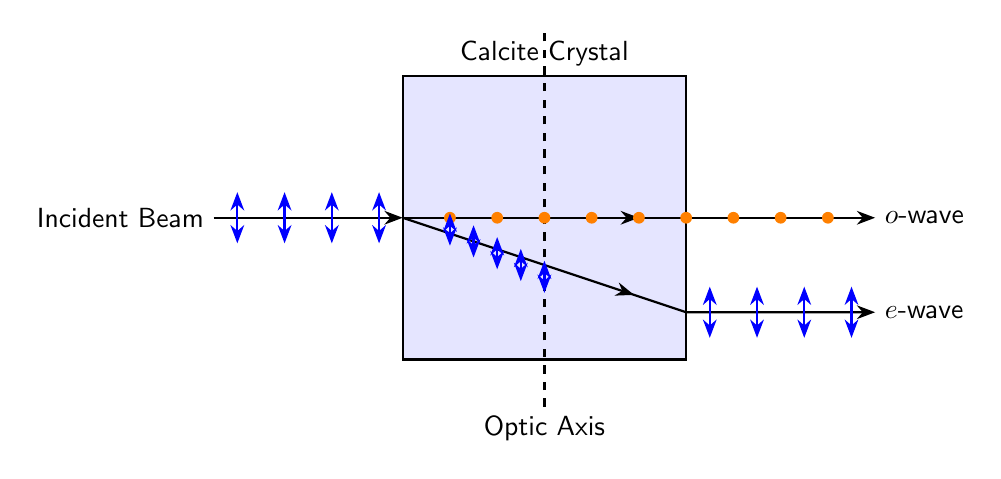
\begin{tikzpicture}[
    scale=1.2,
    >=Stealth,
    every node/.style={font=\sffamily},
    wave/.style={decoration={markings, mark=at position #1 with {\arrow{>}}}, postaction={decorate}},
    polarization/.style={blue, thick, <->, shorten >=1pt, shorten <=1pt},
    dot/.style={fill=orange, circle, inner sep=1.5pt}
]

% Crystal
\fill[blue!10] (0,0) rectangle (3,3);
\draw[thick] (0,0) rectangle (3,3);
\node[above] at (1.5,3) {Calcite Crystal};

% Optic Axis (dashed line)
\draw[dashed, thick] (1.5, -0.5) -- (1.5, 3.5);
\node[below] at (1.5, -0.5) {Optic Axis};

% Incident Beam
\draw[->, thick] (-2,1.5) -- (0,1.5);
\node[left] at (-2,1.5) {Incident Beam};
% Polarization arrows for incident beam
\foreach \x in {-1.75,-1.25,-0.75,-0.25} {
    \draw[polarization] (\x,1.5) ++(0,-0.3) -- ++(0,0.6);
}

% O-wave (ordinary ray)
\draw[->, thick, wave=0.5] (0,1.5) -- (5,1.5);
\node[right] at (5,1.5) {$o$-wave};
% Dots along o-wave
\foreach \x in {0.5,1,1.5,2,2.5,3,3.5,4,4.5} {
    \node[dot] at (\x,1.5) {};
}

% E-wave (extraordinary ray)
\draw[->, thick, wave=0.5] (0,1.5) -- (3,0.5) -- (5,0.5);
\node[right] at (5,0.5) {$e$-wave};
% Polarization arrows for e-wave after crystal
\foreach \x in {3.25,3.75,4.25,4.75} {
    \draw[polarization] (\x,0.5) ++(0,-0.3) -- ++(0,0.6);
}

% Polarization arrows inside crystal for e-wave
\foreach \x in {0.5,1,1.5,2,2.5} {
    \draw[polarization] (0.5*\x + 0.25, 1.5 - 0.25*\x) ++(0,-0.2) -- ++(0,0.4);
}

\end{tikzpicture}

\end{document}